\newpage
\section{Accessible}

The data is considered accessible by the user when he does not need to make an excessive effort to
to be able to obtain them, understand them and use them, that is, apply them to their particular situation. To achieve these objectives,
it is necessary that the user can access them in a way that is familiar and in a language and nomenclature
he can understand.\\ 

So how do we consider that data is accessible to a user?
\begin{itemize}
\item When it is easy to obtain.
The data should be readily available over the web.
\item When it is easy to understand.
The data must be represented in such a way that it's meaning is clear and obvious to a non-specialist. 
Imagine a science writer explaining a complicated concept for a mass market magazine audience. Use everyday language and easily interpretable diagrams.
\item When it is easy to use.
A user must be able to apply the data to their own particular purpose without complicated procedure.
\end{itemize}

In this section we will see if it is possible to access data by an average user and how to optimize accessibility.

% The data itself
\subsection{Interpretabilidad}
The platforms provide a huge volume of data, since, as mentioned earlier, they collect as much data as possible.
There will be multiple samples containing the specified set of fields. These field sets may be similar to each other but don't need to be identical.
From this data, we need to select the relevant samples, and from these, the fields necessary to represent specific information.


Below we can see examples. The first one is taken from the European open data portal
(https://www.eea.europa.eu/data-and-maps/data/air-pollutant-concentrations-at-station/air-pollutant-concentrations-201) and the second from the North American open data portal
(https://data.cityofnewyork.us/api/views/kku6-nxdu/rows.json?accessType=DOWNLOAD).

\begin{figure}[h]
    \centering
    \subfigure[EEUU Open Portal.Demographic Statistics By Zip Code]
     {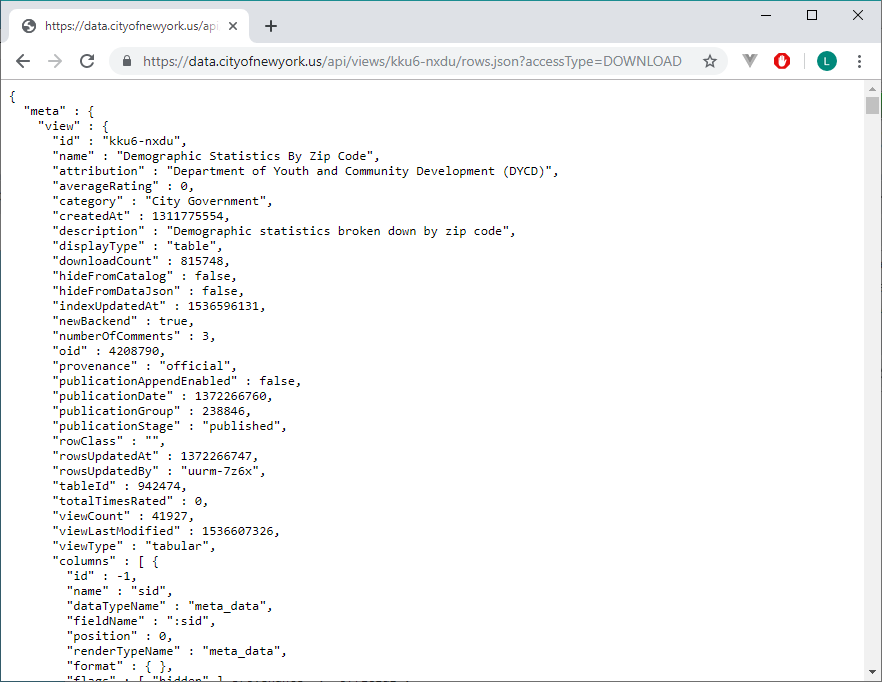
\includegraphics[width=5cm]{ExampleOpenDataEEUU}}
    \hfill
     \subfigure[European Open Data Portal. Air pollutant concentrations 2015]
    {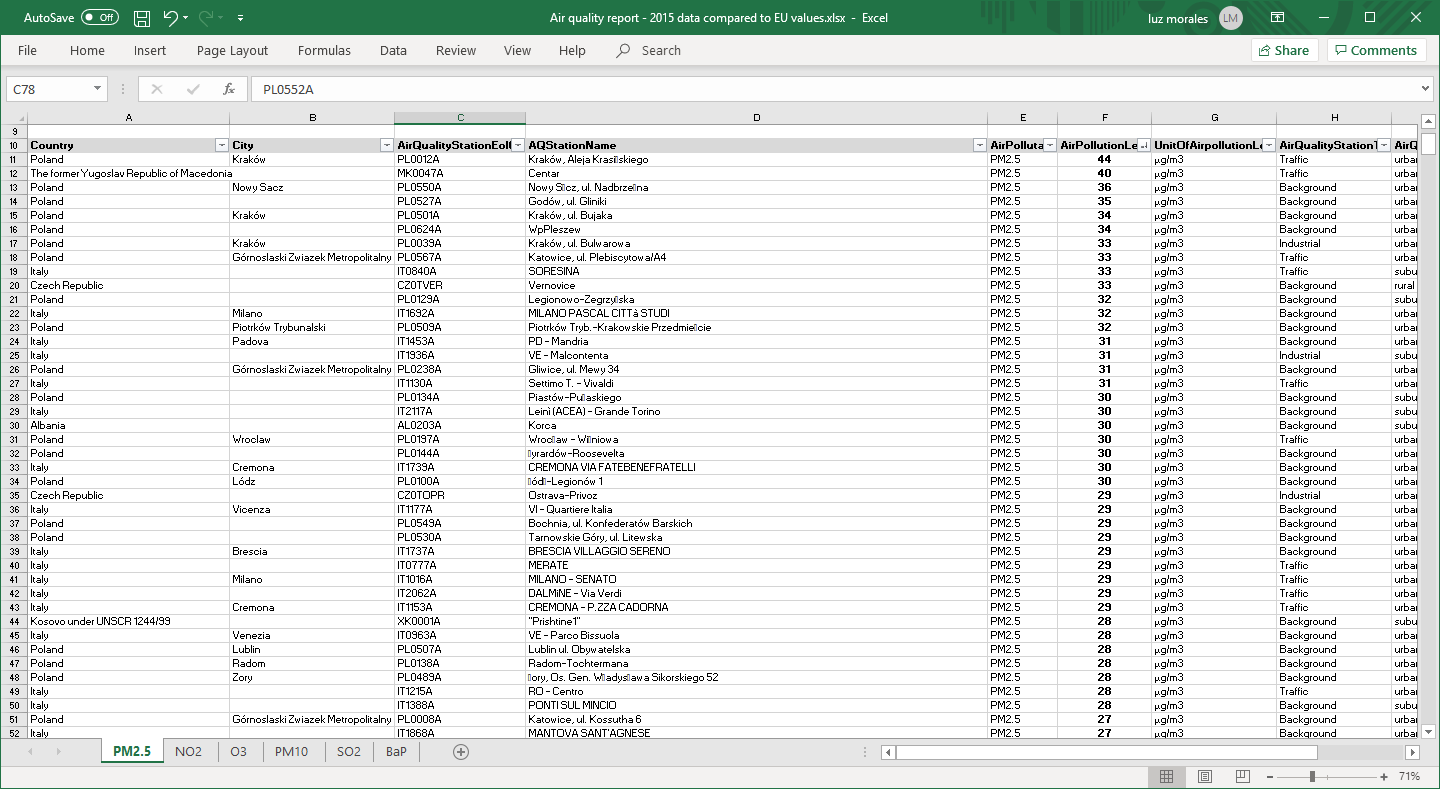
\includegraphics[width=7cm]{ExampleOpenDataEuropean}}
    \caption{Open Data Examples}
\end{figure}

    

    
\subsubsection{How to solve it} 
We obtain our required data through a series of processes such as extraction, transformation and
cleaning of the data. Without automation, theses processes are tedious and time consuming. 

\subsubsection{How we solve it. Aire Guru} 

The extracted data is in GeoJSON format, a format which provides a JSON object with nested subdocuments. Each of these
subdocuments contains a set of data in key-value form.
In the following figure we can see the beginning of the document downloaded on June 9, 2019
(https://datosabiertos.malaga.eu/recursos/ambiente/calidadaire/calidadaire.json)\\
\newpage
\begin{figure}[h]
    \centering
   \subfigure[First subdocument]{ \centering 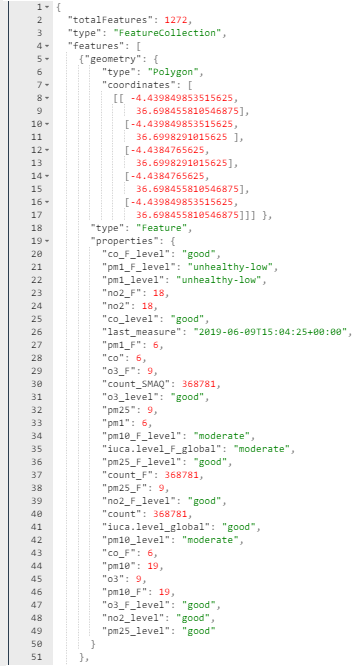
\includegraphics[width=4.75cm]{geoJsonAirQualityData1}}
   \hfill
   \subfigure[Second subdocument]{ \centering 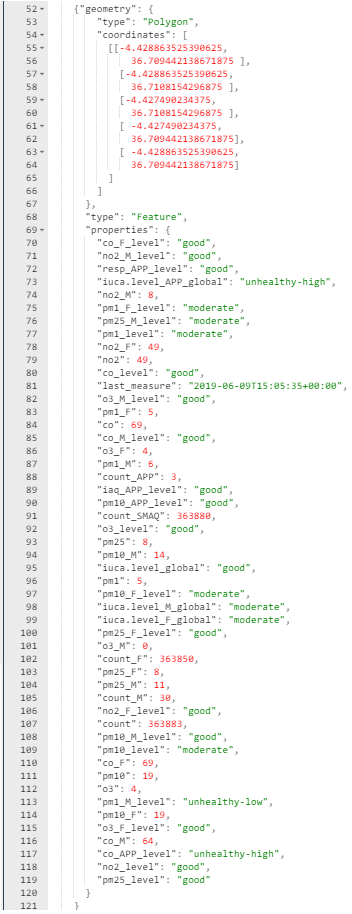
\includegraphics[width=4.75cm]{geoJsonAirQualityData2}}
 
    \caption{Air quality Document [09/06/2019].Open Data Portal Málaga}
    \end{figure}
    
    In this excerpt we can see the first two subdocuments. Each subdocument contains the coordinates of the air quality 
    measuring station, the date and time when the measurement was recorded, and the values of the measurements.
    In the following figure we can find the description provided by the open data portal.
\begin{figure}[ht]
    \centering
    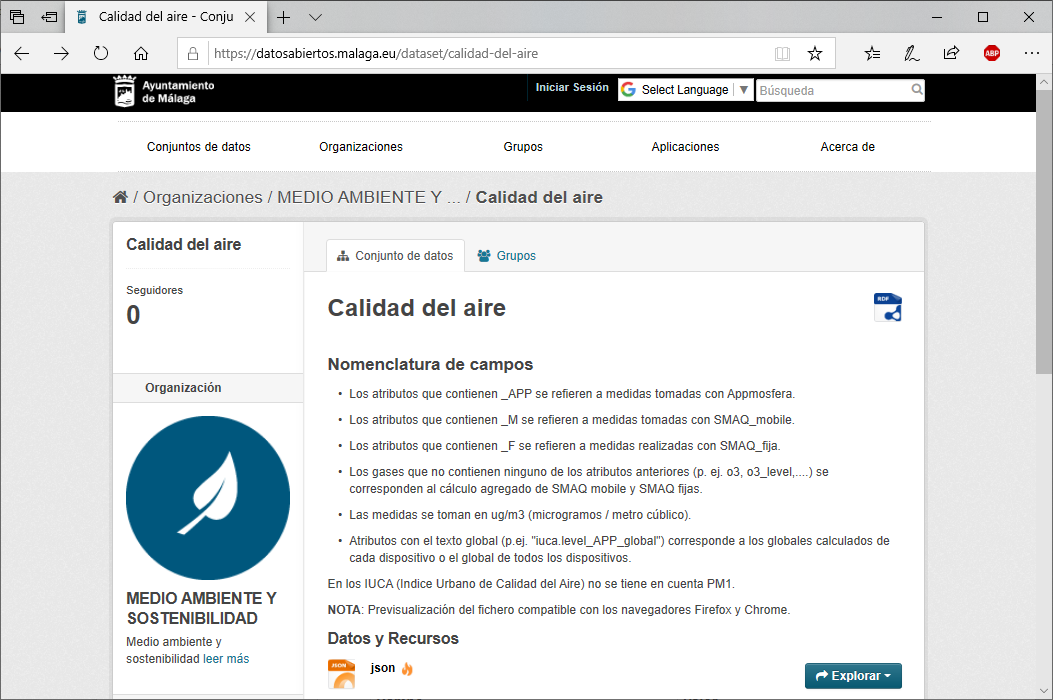
\includegraphics[width=8cm]{geoJsonAirQualityDataDescription}
    \caption{Air quality data description [09/06/2019].Open Data Portal Málaga}
\end{figure}


For a more detailed description of the measures, we have to resort to an external resource. In this case we directly contacted 
the company that installs the UrbanClouds (https://urbanclouds.city/es/) measuring stations and provides the data 
to the Málaga city council.

After selecting the necessary fields according to our design plan, we carried out different cleaning, transformation and extraction tasks. \\


\textbf{Cleaning}. We need to eliminate the repeated or non-relevant fields. For example, the identifier of the measuring station is 
unneccessary as the  already contains the coordinates of the station, and coordinate representation is more interesting for our purposes. \\

\textbf{Transformation}. We need the values to have a format appropriate to the fields that they represent. For example, the date and time 
of the measurement is stored in date format
instead of the string provided in the raw dataset. \\

\textbf{Extraction}. We need to select the relevant fields. This dataset offers one or more measurements for each pollutant, which can be 
represented by three different fields, a
quantitative measurement, a qualitative of the fixed station of measurement and a qualitative station of a mobile station. We will add a 
field containing the measurement which is most relevant for our purposes, and eliminate the non-relevant measurerments to minimize processing time. \\

For security, a second totally independent architecture has been implemented that collects and stores the raw data.

\paragraph{Evaluation} \mbox{} 
\begin{itemize}
    \done We can understand exactly what each one of the fields represented in the dataset means thanks to the 
         complementary information presented in the open data portal and by the complementary information provided by the company in charge of
         collect the data.
    \done The data needed for our model has been extracted from the raw data.
    
\end{itemize}
\newpage

\subsection{Modelo}

Recall that the main objective of accessing the data is to obtain knowledge, to understand and make sense of it. Of course, 
pure data by itself has no value until we can understand it and apply it. We must contextualize, process, and analyze the 
information to gain useful knowledge. \\
    
\begin{figure}[ht]
    \centering 
    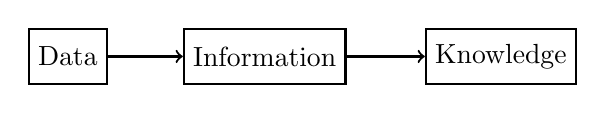
\begin{tikzpicture}[thick]
        \node[draw,rectangle,minimum size=20] (a) {Data};
         \node[draw,rectangle,minimum size=20,right of= a, node distance=2.5cm] (b) {Information};
         \node[draw,rectangle,minimum size=20,right of=b, node distance=3cm] (c) {Knowledge};
         \draw[->] (a) to (b);
        \draw[->] (b) to (c);
     
      \end{tikzpicture}
      \caption{Diagrama. De datos a conocimiento}
    \end{figure}
 
    In order to obtain this knowledge, the user must correctly interpret the data. It's not enough to know what the values and 
    units individually represent, but what they mean in the big picture. For that the user must already have expertise in the 
    area, or must engage in further research allowing them to understand the data that has been extracted.
     
    In order to build a system that makes data accessible, it is essential to design a model to specify the
    information that we want to obtain. The design of a system will allow that, based on given values, provide some results.
    For this it will be necessary to have a solid knowledge of the dataset that is needed, the values,
    their units and how they relate to each other.


\subsubsection{How to solve it} 
Study the objective sought and resort to the help of experts if necessary to acquire the necessary knowledge
on the subject. Design a model that provides the information we are looking for.

\subsubsection{How we solve it. Aire Guru} 
Aire Guru aims to increase the awareness of the level of pollution that surrounds us. To do this, it uses a measure called
the air quality index (AQI), specifically the European air quality index (EAQI).


\newpage
\begin{figure}[ht]
    \centering
    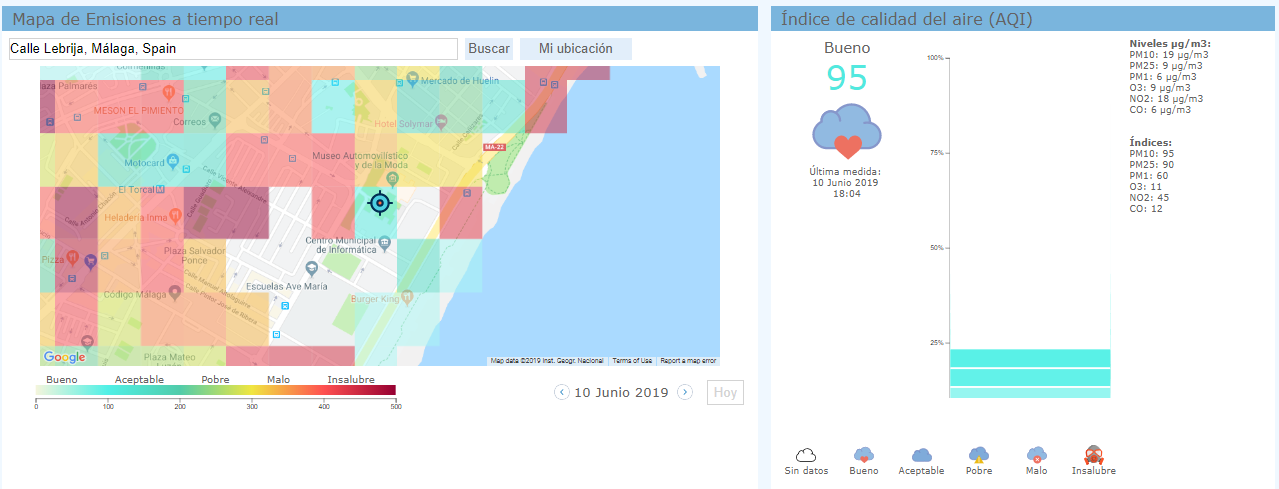
\includegraphics[width=10cm]{mapAireGuru}
    \caption{Aire Guru. Landing page. Top section}
\end{figure}

It shows the AQI in the whole city of Málaga by zones, both the general and the AQI of each of the 
pollutans in a more disaggregated form from September 2018 to the present. It also shows the evolution
of these for days, months and years.
It is capable of creating a set of the most relevant pollutans by medical condition. An innovative feature is the capacity to display levels of any particular pollutant by hour, day, month, or year. 

\elsparagraph{Evaluation}  

\begin{itemize}
\done The information is focused on an objective, informing the user of the level of pollution that surrounds them, both  in real time
and in the past.
\done The information follows a logical thread; it tells a story.
\done The web offers understandabl, useable information, not just raw data.
\end{itemize}

\newpage
\subsection{Formato}
The key point is that the user must be able to understand what we are trying to transmit. We must create a fluid, 
easy interaction between the user and the representation of the data. Therefore we must speak with the language of 
the ordinary person, using common vocabulary, avoiding specialist jargon and communicating the objective in the simplest, 
clearest manner. This representation of information plays a fundamentally important role, enabling the user to absorb 
the meaning in a natural way.



\subsubsection{How to solve it} 
Consider what type of representational format is most appropriate to the task. If it is not possible, we will provide de 
resources needed to help the user to understand and place the information in context. 

We should stady which type of graphs fits better to which kind of data,A graph may not necessarily be the 
clearest way to represent information.

We should take into account the target audience, and how we can most effectively transmit information to them. 
If we decide that a using graph is the best solution, we must consider carefully which type to use. For example, 
if we talk about samples and we want to know the density, we will lean towards a density graph, and if we look for the difference
between sexes, we will use a pie chart.

\subsubsection{How we solve it. Aire Guru} 
The Aire Guru tool presents the information in the native language of the city, using simple vocabulary and a 
straightforward style.
Colors and graphic resources are used as icons. In addition, a unified design structure to represent data has 
been used over the whole site, giving the user a consistent visualization experience. 

One of the objectives is to represent pollution by areas of the city, which is why a map has been used - the 
obvious and familiar visual image of the different places in the city. This is a more legible format since the user
does not need to make a continous effort to place the data in each part of the city. The index shows an indicator with 
five levels represented by a color scale from the turquoise to red ("Good" "Fair" "Poor" "Bad" and "Unhealthy"). 
The color-coding is consistent with the colors which are used in official sources, thereby avoiding onfusion any 
user who might consult official sources.
 \newpage
 \begin{figure}[ht]
    \centering
    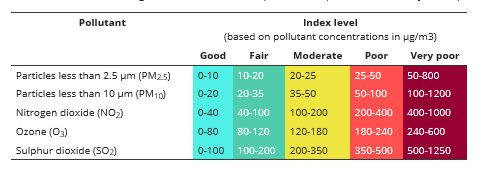
\includegraphics[width=12cm]{EAQI}
    \caption{EAQI Levels}
\end{figure}

These icons below are used to help the user have an immediate idea of the situation, since they are even more
decriptive and self-explanatory than just colors alone. Danger is, of course, almost universally indicated by 
the colour red, and is therefore used appropriately. However, no all cultures has the same perception about
the blue or green, missing what they indicate\\
\begin{figure}[ht]
    \centering
    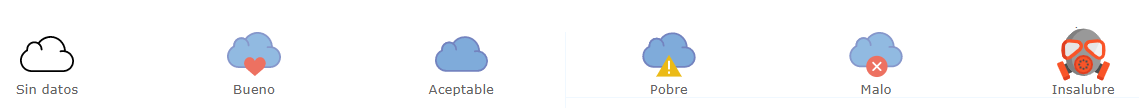
\includegraphics[width=10cm]{EAQI_Icons}
    \caption{Iconografica Aire Guru}
\end{figure}

For the graphs that show variations in time,  we have chosen line graphs as being most appropriate,
since they show the continuous evolution over a period of time. To represent the different components of the AQI, we chose a
graph of stacked bars, since it is easy to see what proportion of the total AQI is formed by which pollutant. \\
\begin{figure}[ht]
    \centering
    \subfigure[AQI Evolution]
     {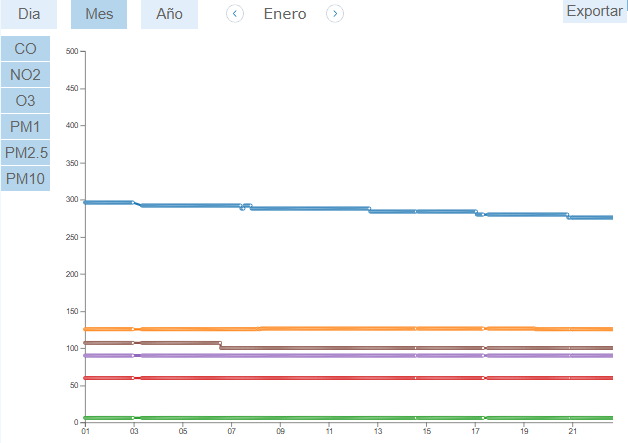
\includegraphics[width=5.75cm]{lineChart}}
     \hfill
     \subfigure [AQI components]
    { 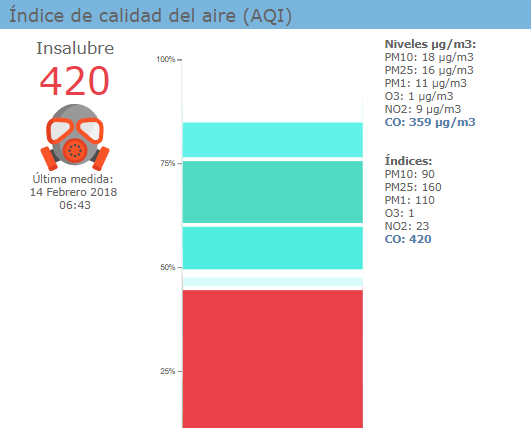
\includegraphics[width=5.25cm]{stakedBarChart}}
 
    \caption{Charts}
\end{figure}

In addition, to explain the concept of AQI and create an awarnes about the influence that air pollution has on us, Aire Guru provides a
glossary. This aids understanding of why air pollution should matter to us, with descriptions of the pollutants, medical complications, sources of contamination, the iconography used and
an explanation of what AQI is and how it is calculated. \\

 
\elsparagraph{Evaluation}  
\begin{itemize}
    \done The language used in the whole tool is a common language, avoiding the use of difficult scientific terminology but providing clearly described information to understand the situation.
    \done The most appropriate graphs for each type of data have been researched and chosen.
    \crossed Some specific terms could not be substituted as "Air Quality Index".
    \done The tools necessary to understand the concept have been provided. The European standard of air quality has been used to
         represent the values and offer the user resources on the page for their comprehension in addition to external resources.
\end{itemize}
 

\newpage

% Access to the data
\subsection{Availability}
    
As we mentioned in the introduction to this chapter, the dataSets may be available in the original source. However, this doesn't necessarily
mean that they are readily accessible.
The challenges we encounter with the raw data direct from the source of origin, are the following: \\   
 
\textbf{Location}. DataSets are usually available in open data portals that have been organized and structured in particular ways.
Despite more companies attempting to offer functional and efficient user interfaces, often a complicated search and selection process is necessary for a user to find what they need. Sometimes the data may not all be available in the one location, but may require searching through multible portals.
\textbf{Extraction}. DataSets are usually available through an API (Application Programming Interface). APIs are not easily interpretable by the average user. Normally there will be a document describing the fields and values presented, and indicating how to actually use the API. \\

\textbf{Readability}. DataSets are usually represented in a format designed to be processed by software. This is fairly unintelligible to a human user. At best,
the data will be represented in a table and even then, it will often be quite difficult to extract the required information.

Therefore, we can not say that data interfaces are commonly accessible in a useful way for the average user. \\

\subsubsection{How can we solve the problem?} 

We must provide the information required by the user in an uncomplicated manner, in a format that is easy to read and interpret, and we must describe it in a way that is easy to understand and quick to digest..

In order to collect the information which is relevant to the user, we will need to carry out processes such as extraction, transformation and
data cleaning.
 
\subsubsection{How we solve it using Aire Guru.} 

Our tool uses the air quality data provided by the city of Malaga in its open data portal.\footnote{\url{https://datosabiertos.malaga.eu/}}\\
\begin{figure}[ht]
    \centering
   \subfigure[Main page]
    {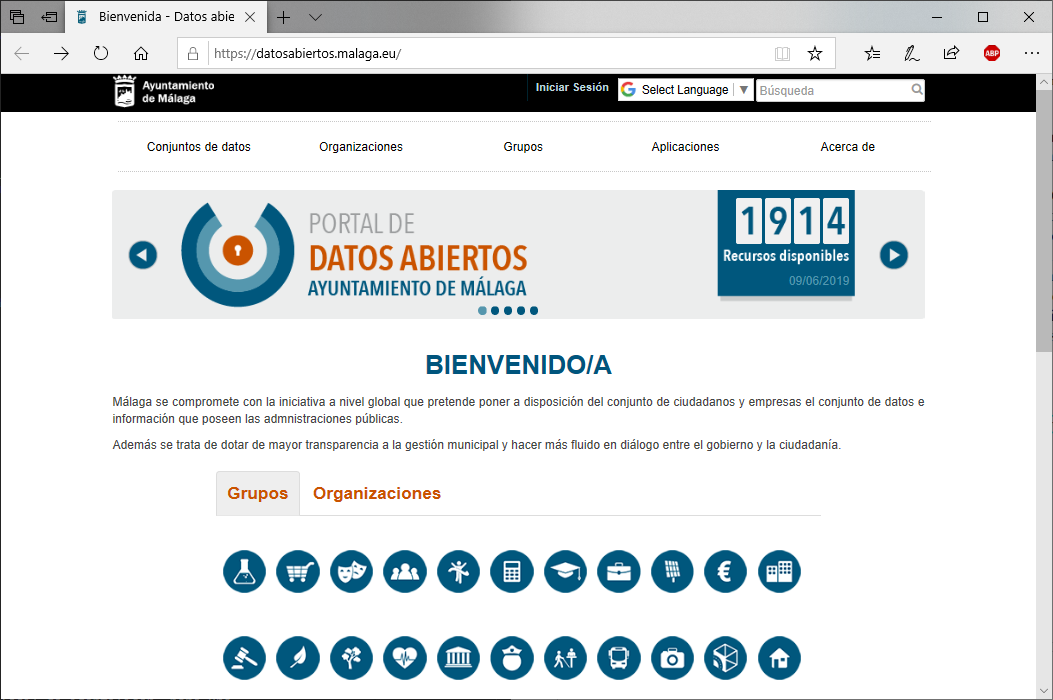
\includegraphics[width=5.5cm]{openDataPortal}}
    \hfill
    \subfigure [Category environment]
       { 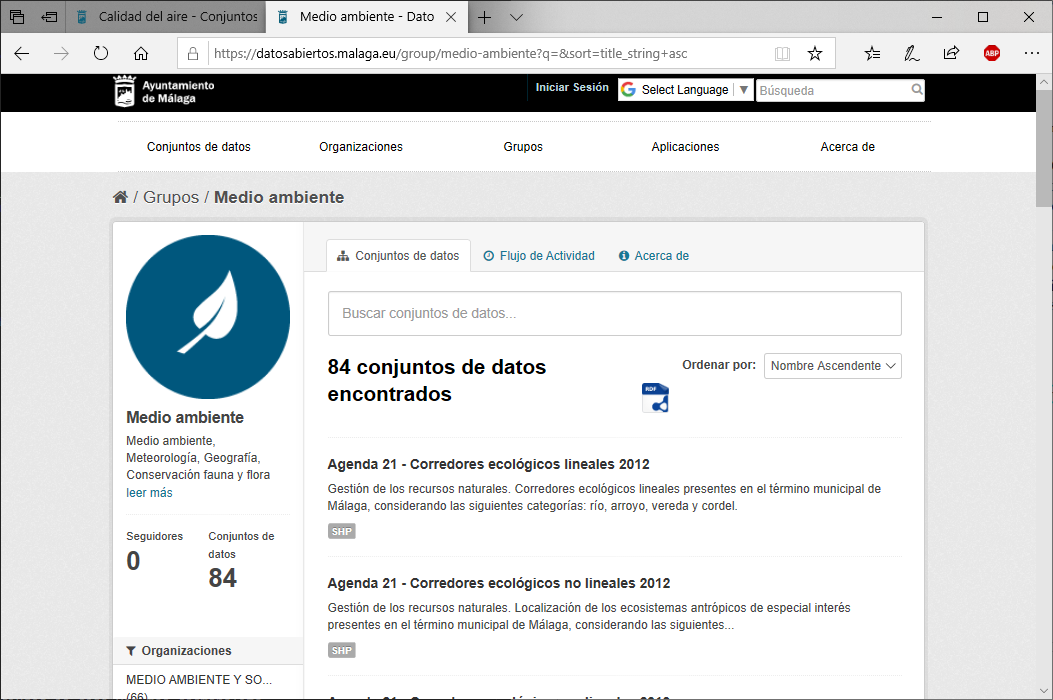
\includegraphics[width=5.5cm]{openDataPortalEnviromentCategory}}




    \vfill
     \subfigure[GeoJson Document]
     { \centering 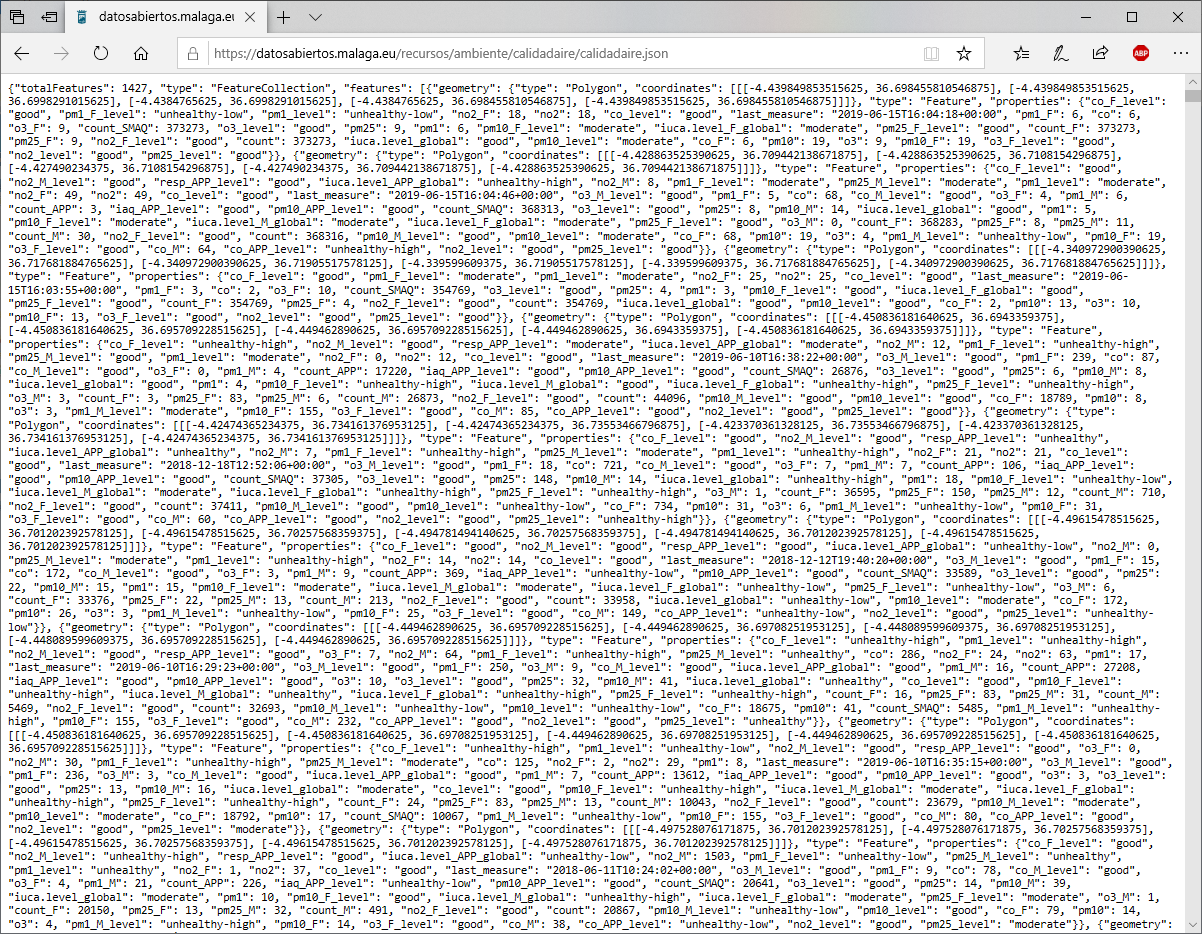
\includegraphics[width=4.75cm]{geoJsonAirQualityDataRaw}}
  
  \caption{Open Data Portal Malaga}
    \end{figure}

    This data portal offers a variety of categories (represented by different icons) indicating classifications of the dataset.
    Once a category is selected, the user is presented with a search bar that allows them to search for specific data using keywords.\\
    
    In this case, if we click on the link, data is displayed in a new tab. The use of software
    for translating the data is not strictly necessary, but we can see that the format (JSON) is not easily readable in human terms.

Aire Guru \footnote{\url{https:\\aire.guru}} offers all the necessary information on a web platform which has been designed to facilitate human understanding.

\elsparagraph{Evaluation}  

\begin{itemize}
    \done Location. Finding data is made simple, since information is displayed immediately on accessing the website. The main page
         presents the levels of pollution in all areas without the need to make any selection.
    \done Extraction. No specialist software or computer knowledge is necessary to access the information.
    \done Readability. Aire Guru includes a map which shows pollution levels, represented by different colors. These colors are defined by a legend
         below the map. It also includes a glossary explains the concepts presented on the website, the meaning of each section and includes clear instructions on how to
         use and navigate through the web page.
 

\end{itemize}
\newpage

 



\subsection{Convenience}
As we mentioned earlier, our goal is for the user to have direct access to the data without having to deal with any
of the technical processes involved in implementing a collection system. The points we must cover to achieve this goal are: \\

\textbf{Infrastructure}. Data collection, processing, storage and visualization. For example, in most cases, the data is
published periodically, but the set of published data only contains the most recent samples. There is no way to obtain
a history of the data if it is not collected, processed and stored periodically. \\

\textbf{Automation}. As we commented in the previous point, these tasks are repetitive and arduous processes, so it will be
necessary to automate, otherwise the effort required by the user to extract the information is not worthwhile. \\

\textbf{Availability} To offer the information to users in a direct way, we should use a platform with which the user is already 
familiar. For example, it is more likely that the user will want to access the data if there are no extra obstacles such as needing 
to install new software on their devices. \\

\subsubsection{How to solve it} 
We will have to provide all the afore-mentioned infrastructure which can collect the data and offer it to the user in an accessible, relevant and compelling way.
We will try to free the user from repetitive actions, we will automate all possible processes, to make the information available immediately.
We must offer the information through a platform with which the user is familiar, nowadays the use of websites or mobile applications is very common.
We must not make the user perform complicated steps, or require them to add extra software or hardware.

\subsubsection{How we solve it. Aire Guru} 
Malaga's air quality dataset is updated every hour, Aire Guru automates the process of collecting the
data through a CRON job that executes a script implemented in JavaScript periodically. This reads the data from the url, processes it,
cleans and stores it in a MongoDB database. That is to say, Aire Guru implements all the necessary collection processes.

Thanks to this infrastructure, the user is able to visualize the evolution of pollutants since 2018. The user can also track their personal exposure
 to these pollutants over the same period of time.

In addition, this automation allows the user to visualize the pollution in the city of Málaga in real time, and see specifically the location where he is 
occurring. \\
\newpage

\begin{figure}[ht]
    \centering
    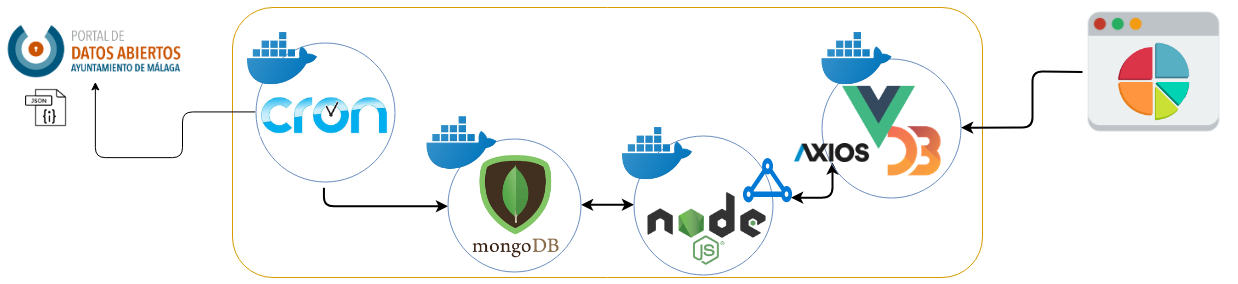
\includegraphics[width=12cm]{aireGuruArquitecture}
    \caption{Arquitecture Aire Guru}
\end{figure}

The data to the users through a web interface. \\

\begin{figure}[ht]
    \centering
    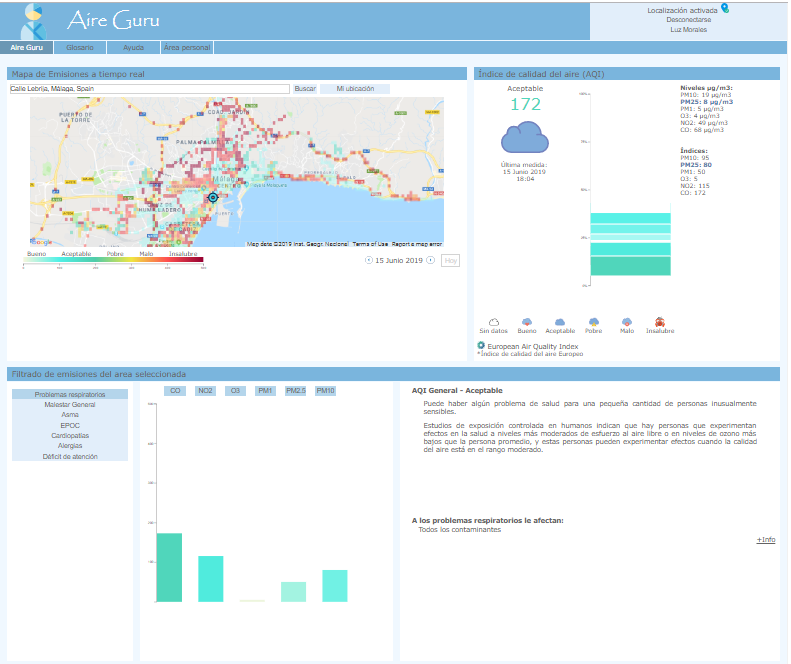
\includegraphics[width=9cm]{aireGuru}
    \caption{Aire Guru. Web Interface}
\end{figure}

To enable access by the majority of the population, Aire Guru is available at the web addresses https://www.aire.guru and https://www.airquality.guru.
We use SSL that guarantees the encryption of data through the network and ensure the user has access to it since, as more and more browsers try to protect 
users by only showing pages that use a secure method.

As we commented previously, all users can see the basic information without having to provide any data or identify themselves, without the need to
perform downloads or installations. Today, almost everyone is familiar with web browsing and if we do not force the user to realize extra taks, as 
requiring them to sign in or install extra software, the probability the user uses our platform will be higher. 

\newpage
\elsparagraph{Evaluation}  
\begin{itemize}
\done The data necessary for our model has been extracted from the raw data.
\done Infrastructure. Aire Guru implements all the necessary architecture of storage, processing and visualization so that the user only has to consult
the data.
\done It automates the processes of data collection and the necessary calculations to show the information to the user.
\done It offers users a free web page, and facilitates the users direct access to information.
\end{itemize}


\subsection{Know about}

No matter how optimized the representation of the data is and how available we make it, if users are not aware
 of the existence of the resource, they can not use it.

\subsubsection{How to solve it} 
The best way is to advertise the product in the right media with right format.
\subsubsection{How we solve it. Aire Guru} 
Our tool is implemented for the city of Málaga, so we are currently working to publicize it in this city.
It is currently available in the open data portal in the web site tab (https://datosabiertos.malaga.eu/aplicaciones) \\
Aire Guru participated in the first open data reuse contest organized by the Málaga City Council (http://cemi.malaga.eu/es/novedades/detalle/1-Concurso-de-Reutilizacion-de-Datos-Abiertos-del-Ayuntamiento-de-Malaga)
and was a finalist in the web page category.


\begin{figure}[ht]
    \centering
   \subfigure[Advertising in the open data portal of Málaga]{ \centering 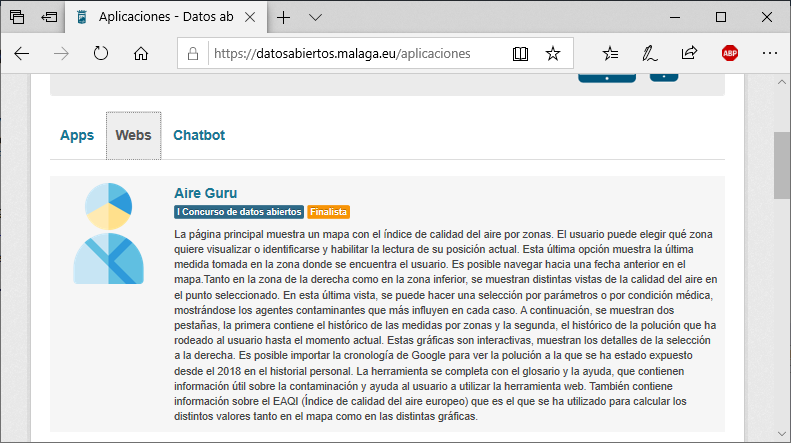
\includegraphics[width=6cm]{aireGuruFinalist}}
   \hfill
   \subfigure[Finalist]{ \centering 
\includegraphics[width=5cm]{aireGuruFinalistCertificate}}
 
    \caption{I Contest of reuse of open data. Málaga's town hall}
    \end{figure}

\elsparagraph{Evaluation}  
\begin{itemize}
    \done It is currently published in the open data portal of the City of Málaga.
\crossed More work should be done on advertising the platform and making it known.
\end{itemize}
\newpage